A utiliza��o de um \textit{Display touchscreen} na interface do usu�rio do novo console para indicadores de destino, tem como objetivo dar uma maior versatilidade e dinamismo a essa interface. Como o  TOPWAY HKT080ATA-C, apresentado na Figura (\ref{fig:DisplayTOPWAY}) � poss�vel instanciar e remover janelas, teclados e bot�es interativos de acordo com a necessidade. 

\vspace{9mm}
\begin{figure}[H]
	\centering
	\captionsetup{width=0.8\textwidth, font=footnotesize, textfont=bf}	
	\includegraphics[width=0.5\linewidth, angle=90]{Images/DisplayTOPWAY.eps}
	\caption{\textit{Display Touchscreen} TOPWAY HKT080ATA-C}
	\vspace{-3.5mm}
	\caption*{Fonte: Autoria Pr�pria}
	\label{fig:DisplayTOPWAY}
\end{figure} 
\vspace{9mm}

O  TOPWAY HKT080ATA-C � um modulo \textit{Smart display} de 7 polegadas TFT LCD (\textit{thin film transistor liquid crystal display}), possui uma interface de comunica��o UART-RS232. Por ser um modulo \textit{Smart} este \textit{display} torna o desenvolvimento mais �gil e simples. O fabricante disponibiliza um programa de edi��o gr�fica de interface, o \textit{TOPWAY TML Graphics Editor}, visto na Figura (\ref{fig:TMLGraphicsEditor}). 

\vspace{9mm}
\begin{figure}[H]
	\centering
	\captionsetup{width=0.99\textwidth, font=footnotesize, textfont=bf}	
	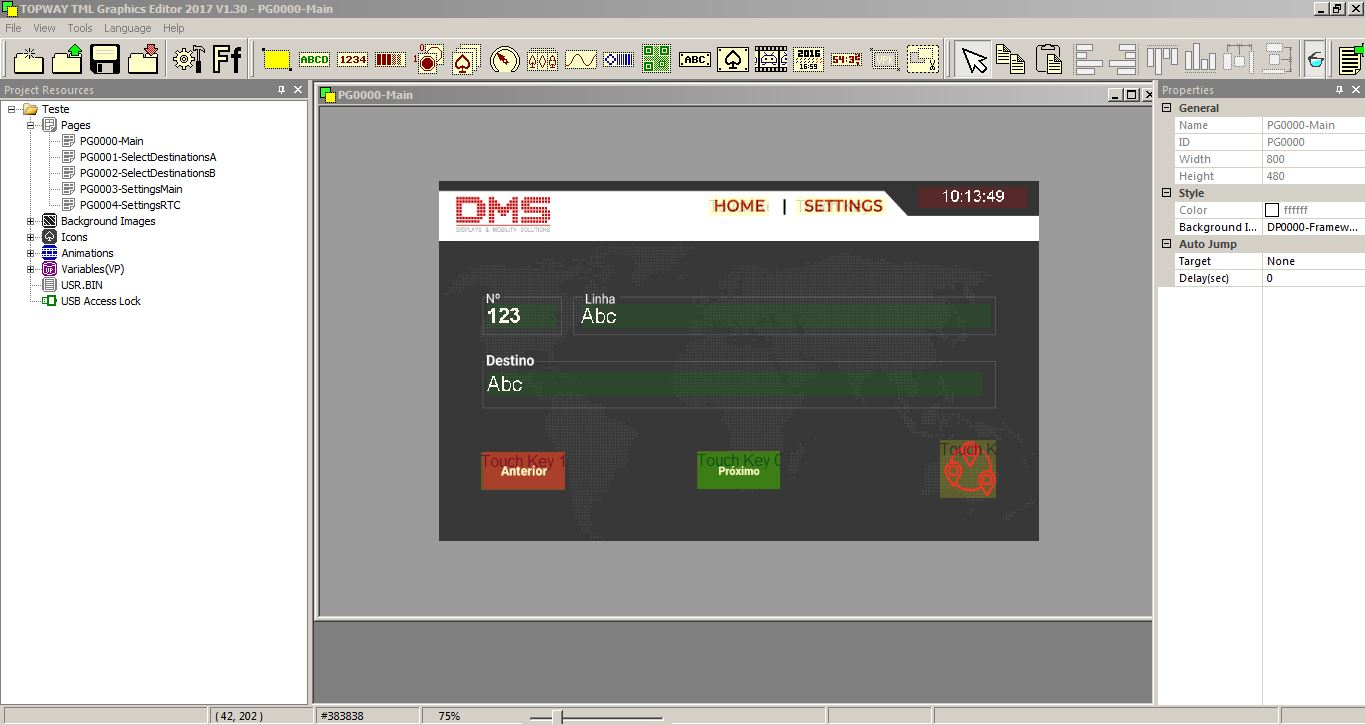
\includegraphics[width=0.99\linewidth]{Images/TMLGraphicsEditor.JPG}
	\caption{Programa de Edi��o de Interface \textit{TOPWAY TML Graphics Editor}}
	\vspace{-3.5mm}
	\caption*{Fonte: Autoria Pr�pria}
	\label{fig:TMLGraphicsEditor}
\end{figure} 
\vspace{9mm}

Por meio desta aplica��o � poss�vel instanciar elementos gr�ficos, configurar comportamentos responsivos, alocar vari�veis que armazenam eventos e configurar gatilhos para transmitir via UART-RS232 as informa��es sobre eventos. Ainda � poss�vel designar �reas de texto na interface, tais �reas s�o preenchidas com informa��es que podem ser enviadas de um dispositivo mestre para o \textit{display} via UART. Assim basta criar os elementos gr�ficos da interface e suas a��es, atrav�s do \textit{TOPWAY TML Graphics Editor}, e gerenciar a interface usando o dispositivo mestre. O dispositivo mestre utilizado neste trabalho � o Raspberry Pi - Zero W. 